%%%%%%%%%%%%%%%%%%%%%%%%%%%%%%%%%%%%%%%%%%%%%%%%%%%%%%%%%%%%%%%%%%%%
%
% IMPERIAL COLLEGE LONDON DISSERTATION TEMPLATE 
%
%%%%%%%%%%%%%%%%%%%%%%%%%%%%%%%%%%%%%%%%%%%%%%%%%%%%%%%%%%%%%%%%%%%%
%
% This file is `icldiss.tex'
%
% This document fulfills the layout requirements for Dissertations
% of the University of London and of Imperial College London.
% To do so it uses the documentclass `icldt' which is provided free 
% of charge under the MIT license. The relevant College regulations,
% and the license are included in the `icldt' manual.
%
% If you print your dissertation for yourself or as a present for
% family, friends or colleagues you probably should use a different
% layout which does not fulfill the College requirements but which
% can look much better.
%
% For further information and for professional layouting and
% printing services please visit www.PrettyPrinting.net
%
% Copyright (c) 2008, Daniel Wagner, www.PrettyPrinting.net
%
%%%%%%%%%%%%%%%%%%%%%%%%%%%%%%%%%%%%%%%%%%%%%%%%%%%%%%%%%%%%%%%%%%%%

\documentclass[MSc]{icldt}

\usepackage{parskip}
\usepackage{amsmath}
\usepackage[latin1]{inputenc}
\usepackage{tikz}
\usetikzlibrary{shapes,arrows}
\usepackage{float}
\usepackage{listings}
\usepackage{color}
\usepackage[T1]{fontenc}
\usepackage{pgfplots}
\usepackage{graphicx}
\usepackage{caption}
\usepackage{subcaption}
\definecolor{dkgreen}{rgb}{0,0.6,0}
\definecolor{gray}{rgb}{0.5,0.5,0.5}
\definecolor{mauve}{rgb}{0.58,0,0.82}

\lstset{frame=tb,
  language=Java,
  aboveskip=3mm,
  belowskip=3mm,
  showstringspaces=false,
  columns=flexible,
  basicstyle={\small\ttfamily},
  numbers=none,
  numberstyle=\tiny\color{gray},
  keywordstyle=\color{blue},
  commentstyle=\color{dkgreen},
  stringstyle=\color{mauve},
  breaklines=true,
  breakatwhitespace=true
  tabsize=3
}

\title{Tree of Life Visualisation \\ By}
\author{Kai Zhong(kz12)}


% Please specify you department here.
\department{Computing}

% The college regulations do not require that you mention 
% your supervisor on the titlepage of you dissertation.
% If you want to do so put her name here.
\supervisor{}
% The college regulations do neither require nor forbid 
% a dedication of your dissertation to somebody or something. 
% If you want to include a dedication put the text here. 
\dedication{}

\date{September 2013}

\begin{document}

\maketitle

\tikzstyle{decision} = [diamond, draw, fill=blue!20, 
    text width=5.5em, text badly centered, node distance=3cm, inner sep=0pt]
\tikzstyle{block} = [rectangle, draw, fill=blue!20, 
    text width=8em, text centered, rounded corners, minimum height=4em]
\tikzstyle{line} = [draw, -latex']
\tikzstyle{cloud} = [draw, ellipse,fill=red!20, node distance=3cm,
    minimum height=2em]
    
\begin{abstract}

The storage, searching and visualisation of big data has become an increasingly important issue in computer science. One technique for visualisation of huge hierarchies is the interactive fractal inspired graph(IFIG), which employs fractal geometry to place limitless amounts of information on a single page and show,or  hide information by the simple actions of zooming and panning. This method has been employed for tree of life visualisation where it solved a significant outstanding problem in evolutionary biology: how can large evolutionary trees be visualised effectively for science, education and public outreach.

While the pre-existing software runs on javascript and html5, the object of this project is to develop an android application based on this code. Compared with a personal computer, the calculation ability of a mobile device is relatively low and the RAM capability is more restricted. The project develops a multi threaded method with cached bitmaps to solve the performance issue. This greatly shortens the loading time as well as the response time of user interaction. When dealing with larger trees, because of the limitation of RAM, dynamical loading and freeing of objects is employed in this project, such that the usage of RAM could be maintained under the limitation of an android application. 
The techniques developed in this project could also be employed to solve performance issues in the website software

\end{abstract}

\chapter*{Acknowledgement}

I would like to thank my supervisor Professor Duncan Gillies for the supports, valuable comments and guidance he provided me throughout my project period.

I also wish to thank Dr.James Rosindell for sharing me the manuscript of the website software as well as providing important advices and comments for the application.


\makededication

\tableofcontents
\listoftables
\listoffigures

\chapter{Introduction}

\section{Background}

\subsection{What is tree of life?}
The tree of life links all biodiversity through a shared evolutionary history. \cite{emotiv}

This project will produce the first online, comprehensive first-draft tree of all 1.8 million named species, accessible to both the public and scientific communities. Assembly of the tree will incorporate previously-published results, with strong collaborations between computational and empirical biologists to develop, test and improve methods of data synthesis. This initial tree of life will not be static; instead, we will develop tools for scientists to update and revise the tree as new data come in. Early release of the tree and tools will motivate data sharing and facilitate ongoing synthesis of knowledge.

Our knowledge of the tree of life, a phylogenetic tree summarizing the evolutionary relationships among all life on Earth--is expanding rapidly. "Megatrees" with millions of tips (species) are expected to appear imminently. Unfortunately, there has so far been no practical and intuitive way to explore even the much smaller trees with thousands of tips that are now being routinely produced. Without a way to view megatrees, these wondrous objects, representing the culmination of decades of scientific effort, cannot be fully appreciated. The field really needs a solution to this problem to enable scientists to communicate important evolutionary concepts and data effectively, both to each other and to the general public.


Visualising phylogenies is one of the fundamental tasks of evolutionary analysis. It has long been a great challenge to display huge trees. When the number of species on the tree increases to millions, no display is huge enough to display the whole tree while maintaining all metadata(e.g., name, population stability, conservation status) of each species. Even if a screen large enough is accessible, it is unpleasant for users to look for information on such a large screen. 

One way to solve this issue is the interactive fractal-inspired graph(IFIG), which includes all species as well as all their metadata. The key concept of the IFIG method is to place all the data on one page such that users could navigate between different scales by simply zooming in and out (http://www.onezoom.org). Therefore, users can't see all information of all species at one time. Instead, when the scale is big enough, users could see the whole picture of the tree of life but with few details of each species. When users zoom into the tree, more details of the selected area will be displayed while other species might go out of the screen.

The interface of the OneZoom is analogous to Google Earth. When using google earth, one can find a location by zooming from a start page of the whole globe, recognizing familiar landmarks at different scales along the way(e.g., continents, countries, regions, and towns)(TODO: add reference). Equivalently, OneZoom enables the user to zoom smoothly to the species they want to find. For example, one can find human beings by zooming in along the clades of animals, vertebrates, mammals and primates.(reference) The hierarchical dataset is represented by using fractals. Fractals are typically self similar patterns, where self similar means they are "the same from near as from far". This means the shapes of branches and nodes remains similar at different scales of zoom.(TODO: add reference) Hence, it could ensure the amount of visual elements on a screen remains relatively constant. Moreover, fractals simplify the representation of huge hierarchical dataset. All levels of data are represented in the same way. So inserting or deleting data can be automatically adopted by the software in the tree representation.

TODO: Duncan suggested to add more background about previous weak and perhaps something more on fractals and self similarity. Besides, Duncan also suggested to add some background about android development environment.



\section{OneZoom Android Application}

The IFIG method was only implemented using javascript and html5. The aim of this project is to develop an android application of it. The application is based on the javascript code written by Dr. James Rosindell. 

When the application was developed, the first issue that arose is that the loading time of a tree is over long. This problem also occurs in the website software, though it is not very obvious due to faster processor of personal computer compared to a mobile device. The fluency of the user interaction is a issue. There were apparent delays when users interacted with the application. Both of these issues have been solved and details of that will be discussed in Chapter 5.

As the data gets larger, more memory needs to be allocated. As the memory one android application can be allocated is quite small, the application sometimes crashes when drawing the tree of tetrapods which has over 22,000 species. This is also a potential issue for the further development of the software on OneZoom website when the size of tree grows to over million species. The more detailed description of this problem the solution of it will be discussed in Chapter 4.



\section{Report outline}

Chapter 2 gives introduction to the software that will be built on. It includes what interactions users could have with this software, the basic structure of the software, what methods are used to increase the performance of the software as well as some functions that will be inherited in the mobile application. Chapter 3 mainly talks about some changes in the implementation of the node class and how the application listens to user interactions. 

 When the dataset gets larger, the application will hit memory limitation. Chapter 4 gives a description of this issue and also the solution for it. Chapter 5 discusses ways to improve the performance of the application. It includes shortening loading time as well as making user interaction more fluent.
 

\chapter{OneZoom Website Software Introduction}

This chapter gives a brief introduction to the OneZoom website software, on which the whole project has been built. It manifests how the raw data is organized and how the member variables of the node object built based on the raw data. Then it explains the criteria for selecting elements to be drawn. These two sections are highly related to the memory issue that will be discussed later. Then an introduction to the software working flow would be given, which is highly related to the performance issue in Chapter 5. Lastly, I will illustrate how to use the software from a user's perspective.

\section{Data Processing}

\subsection{Raw data format}

The raw data is a string in Newick format. In Newick format there are nodes, branch lengths and brackets. For instance, if two species A and B have a common ancestor node C 1.5 million years ago the Newick string looks like this: 
\begin{center}
	(A:1.5, B:1.5)C. 
\end{center}

Then if species D and species C have a common ancestor E 3.5 million years ago, the Newick string becomes: 
\begin{center}
	((A:1.5,B:1.5)C:2,D:3.5)E. 
\end{center}
If this group of species have a further ancestor, then this string will be regarded as a whole and replace A in the first expression to form a larger Newick string. By recursively doing this, a string representing any size of tree can be built.

Building a tree from the string is just the opposite as building the tree. For instance, given the second string, the node E out of the brackets would be first taken out. Then the remainder of the string will be split to two children.

\begin{center}
	"((A:1.5,B:1.5)C:2,D:3.5)E" =  "(" + "(A:1.5,B:1.5)C:2" + "," + "D:3.5" + ")" + "E"
\end{center}

Therefore, a node object E with two children will be built. Its first children need to be further initialized while its second children will be node D. For a larger dataset, building a tree follows the same steps. First create the node out of the outer bracket, then split the data inside the bracket into two parts and set each part to be one of the children of the outer node. Then continue initialising its children by the same steps.

Finally, for any Newick string, a binary tree starting from a root would be built. 

\subsection{Node object}

Basically, the nodes in a Newick string can be categorized into two types, link node(node with children) and leaf node(node without children).

For each leaf node in the Newick string, it contains a species name and the metadata e.g. a node named: Tachyglossus\_ aculeatus\{Short-beaked Echidna\_ LC\_ S\} means that it's the animal 'Tachyglossus aculeatus' (latin name) with common name Short-beaked Echidna and redlist status LC(which means least consern) and population stability S(which means stable). While for the link nodes, it does not contain information of its redlist status and its population stability in the raw data. These two pieces of information in the link nodes are statistics of the redlist status and population stability of all of their children. 

Besides redlist and population stability, the richness of link nodes are also statistic of their children, while the richness of a leaf node is always 1. 

Another metadata that cannot be accessed directly from the raw data is the age of link nodes. The age of the root needs to be inferred from its children. Take the previous string as an example, the node hierarchy can be represented as below. The age of node C is 1.5 million years from either child A or B. While the age of node E is 3.5 million years from child C or D.

\begin{center}
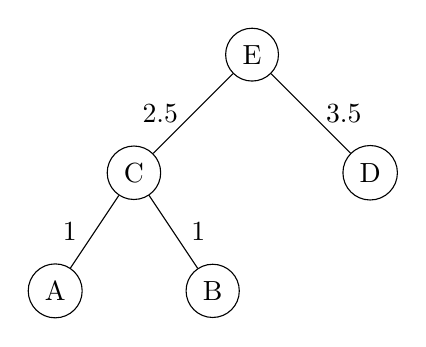
\begin{tikzpicture}[level distance=1.5cm,
level 1/.style={sibling distance=3cm},
level 2/.style={sibling distance=2cm}]
\tikzstyle{every node}=[circle,draw]

\node (Root)  {E}
    child {
    node {C}
    child { node {A} edge from parent node[left,draw=none] {1}}
    child { node {B} edge from parent node[right,draw=none] {1}}
    edge from parent node[left,draw=none] {2.5}
}
child {
    node {D} edge from parent node[right,draw=none] {3.5}
};

\end{tikzpicture}
\end{center}

The data shown above is information about a species, e.g. the name of a species, the richness of a species. 

Apart from the metadata, node objects also contain information about drawing an element. More specifically, this information can be divided into two parts. The first part tells the software where to draw the elements like bezier start, control and end points and how big should the elements be drawn like the branch line width, circle radius. The second part tells the software the bounding box of a node. Each node has two kinds of bounding box, a bigger one representing a bounding box of itself and all of its children and a smaller one representing a bounding box of the node itself. 


\section{Ways to decrease the amount of elements being drawn}

For a tree big enough, not all of the nodes would be drawn at any given time. There are two criteria for selecting elements to be drawn. The first is to compare the size of a node with a threshold. When the size of a node is smaller than the threshold,the node and all of its children should not be drawn. There are also some other thresholds. Both leaf nodes and link nodes could show text. The text can appear or disappear, displaying in greater details or in fewer details. All these are controlled by the relative threshold and the size of these nodes. The second criteria is to test whether the bounding box of a node is within the screen. Here we use the bounding box containing only the node itself. If the node is in the bounding box, then it should be drawn, otherwise it should not. 

\section{Software work flow}

The software first draws a loading page since it might take some time for the full tree being loaded and the loading page tells users that the software is still responding. The loading time increases linearly with the size of the species, which may become unacceptable for larger trees. A reasonable solution for shortening loading time can be found in chapter 4: Performance Issues. 

After drawing the loading page, the software starts creating objects representing tree nodes from data. This is followed by initializing some node information, like the age of some nodes, which cannot be got directly from data but has to be calculated from their children nodes. Then pre calculation is called to calculate the Bezier curve parameter of each node such that the relative position of each node is known. 

When pre calculation is over, the software will call a method to update the view and display the whole tree. From then on, user actions like tap and drag are listened and methods for recalculating the position and scale of node objects will be called. When recalculation is done, the tree will be updated. 

\begin{tikzpicture}[node distance = 6cm, auto]
    % Place nodes
    \node [block] (drawLoading) {Displaying Loading};
    \node [block, below of=drawLoading, node distance = 4cm] (load) {Loading and Pre Calculating};
    \node [block, right of=load, node distance = 5.5cm](update) {Update View};
    \node [block, right of=drawLoading, node distance = 5.5cm] (view) {Displaying Tree};
    \node [block, right of =view, node distance = 5.5cm](operation){Drag or Zoom};
    \node [block, below of=operation, node distance = 4cm](setting){Recalculation or Set Parameters};
    %Draw edges
    \path [line] (drawLoading) -- (load);
    \path [line] (load) -- (update);
    \path [line] (update) -- (view);
    \path [line] (view) -- (operation);
    \path [line] (operation) -- (setting);
    \path [line] (setting) -- (update);
\end{tikzpicture}


\section{How to use the software}
Basically, the OneZoom software allows users to explore the tree of life in a completely new way: it's like a map, everything is on one page, all you have to do is zoom in and out(reference). When a user zooms in, some nodes become visible and more details will be shown on nodes. On the other hand, when a user zooms out, some nodes become invisible and some details will disappear in order to provide the user a neat view. 

For example, in the figure of the tree of mammals, one branch is covered by a signpost rodents. If we zoom in this area, we can see that more signposts appears telling us more details of the rodent family. If we continue zoom in the mouse-like rodents, we can see that nodes that was invisible in the first two figures emerging.

\begin{figure}[H]
  \centering
  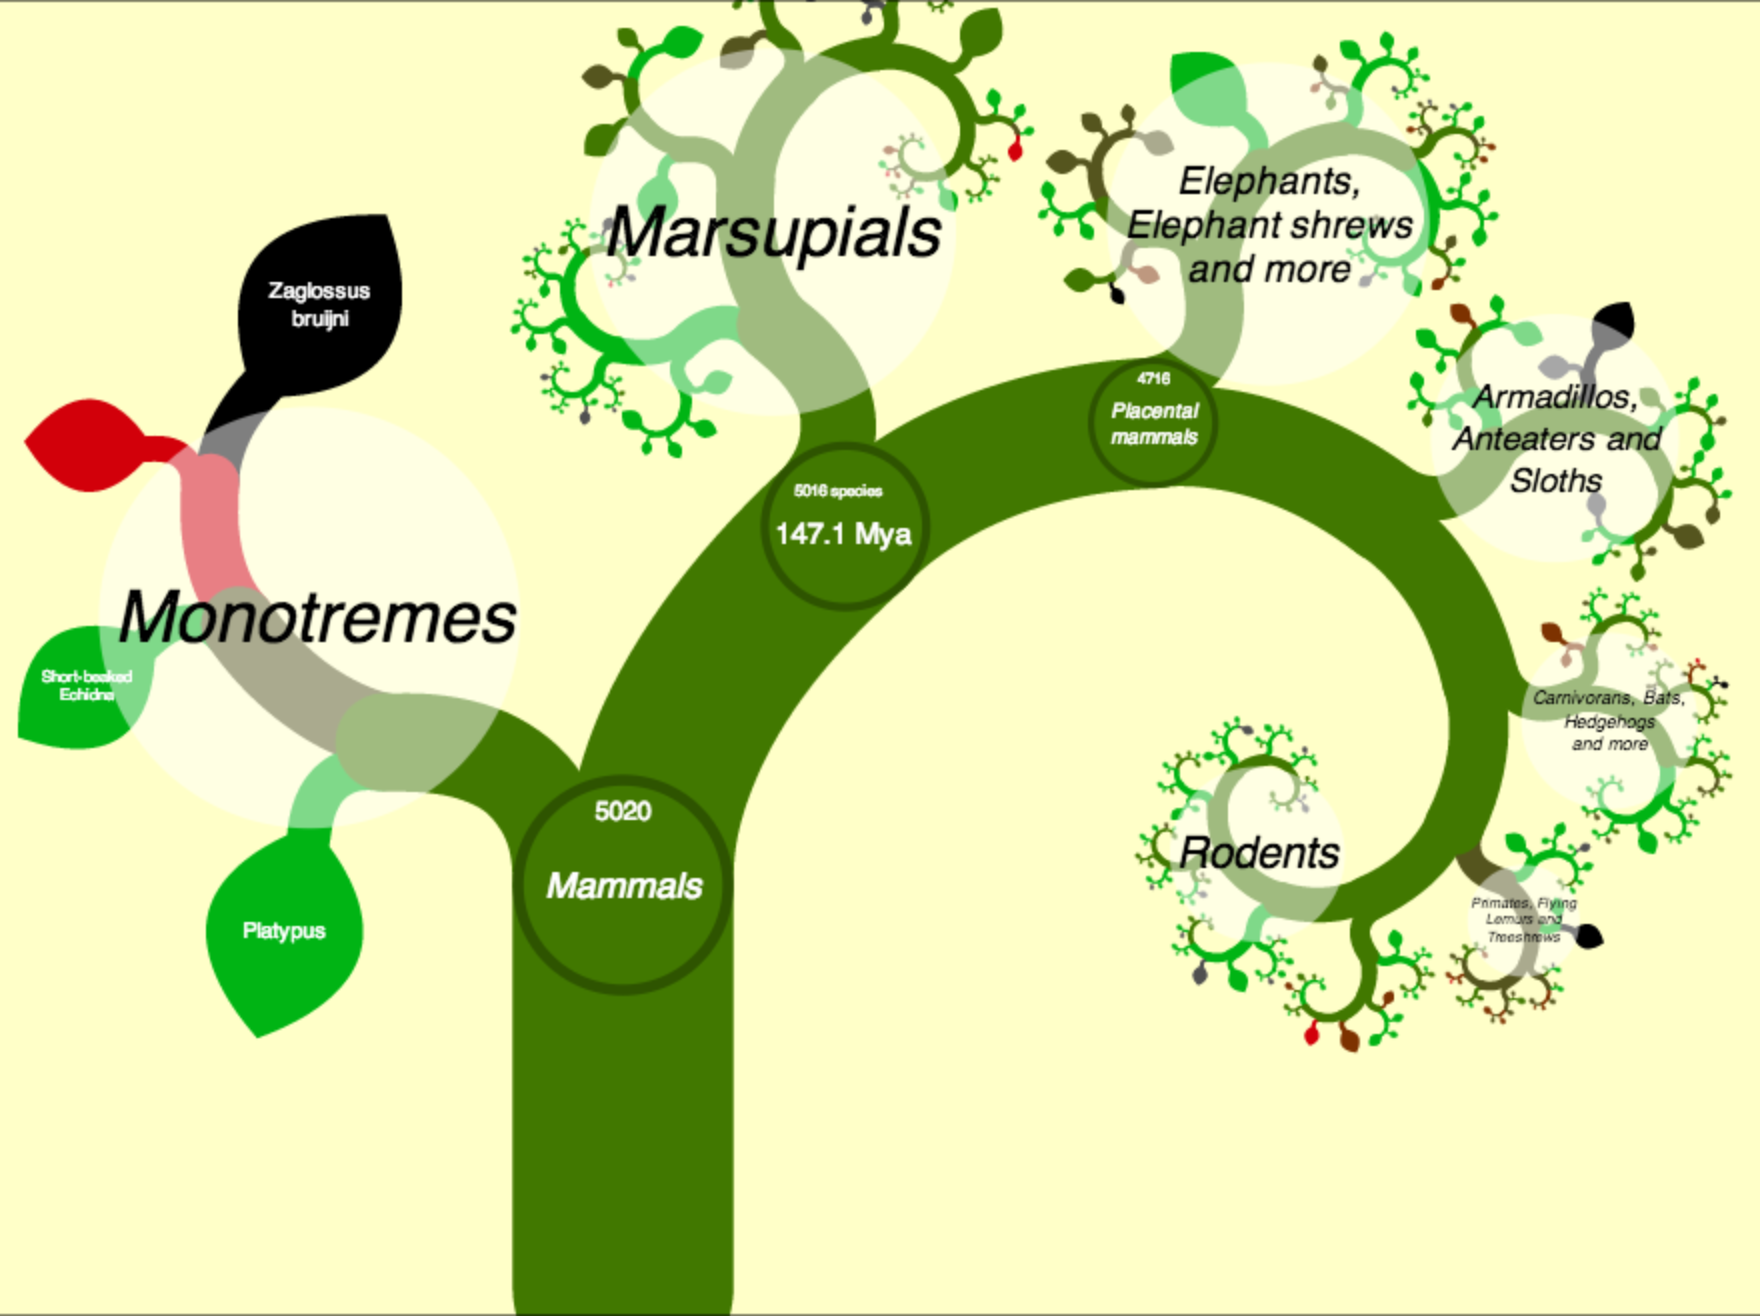
\includegraphics [width=15cm,height=8.8cm]{Mammal}
  \caption{Tree of Mammals}
  \label{fig:mammal}
\end{figure}

\begin{figure}[H]
  \centering
  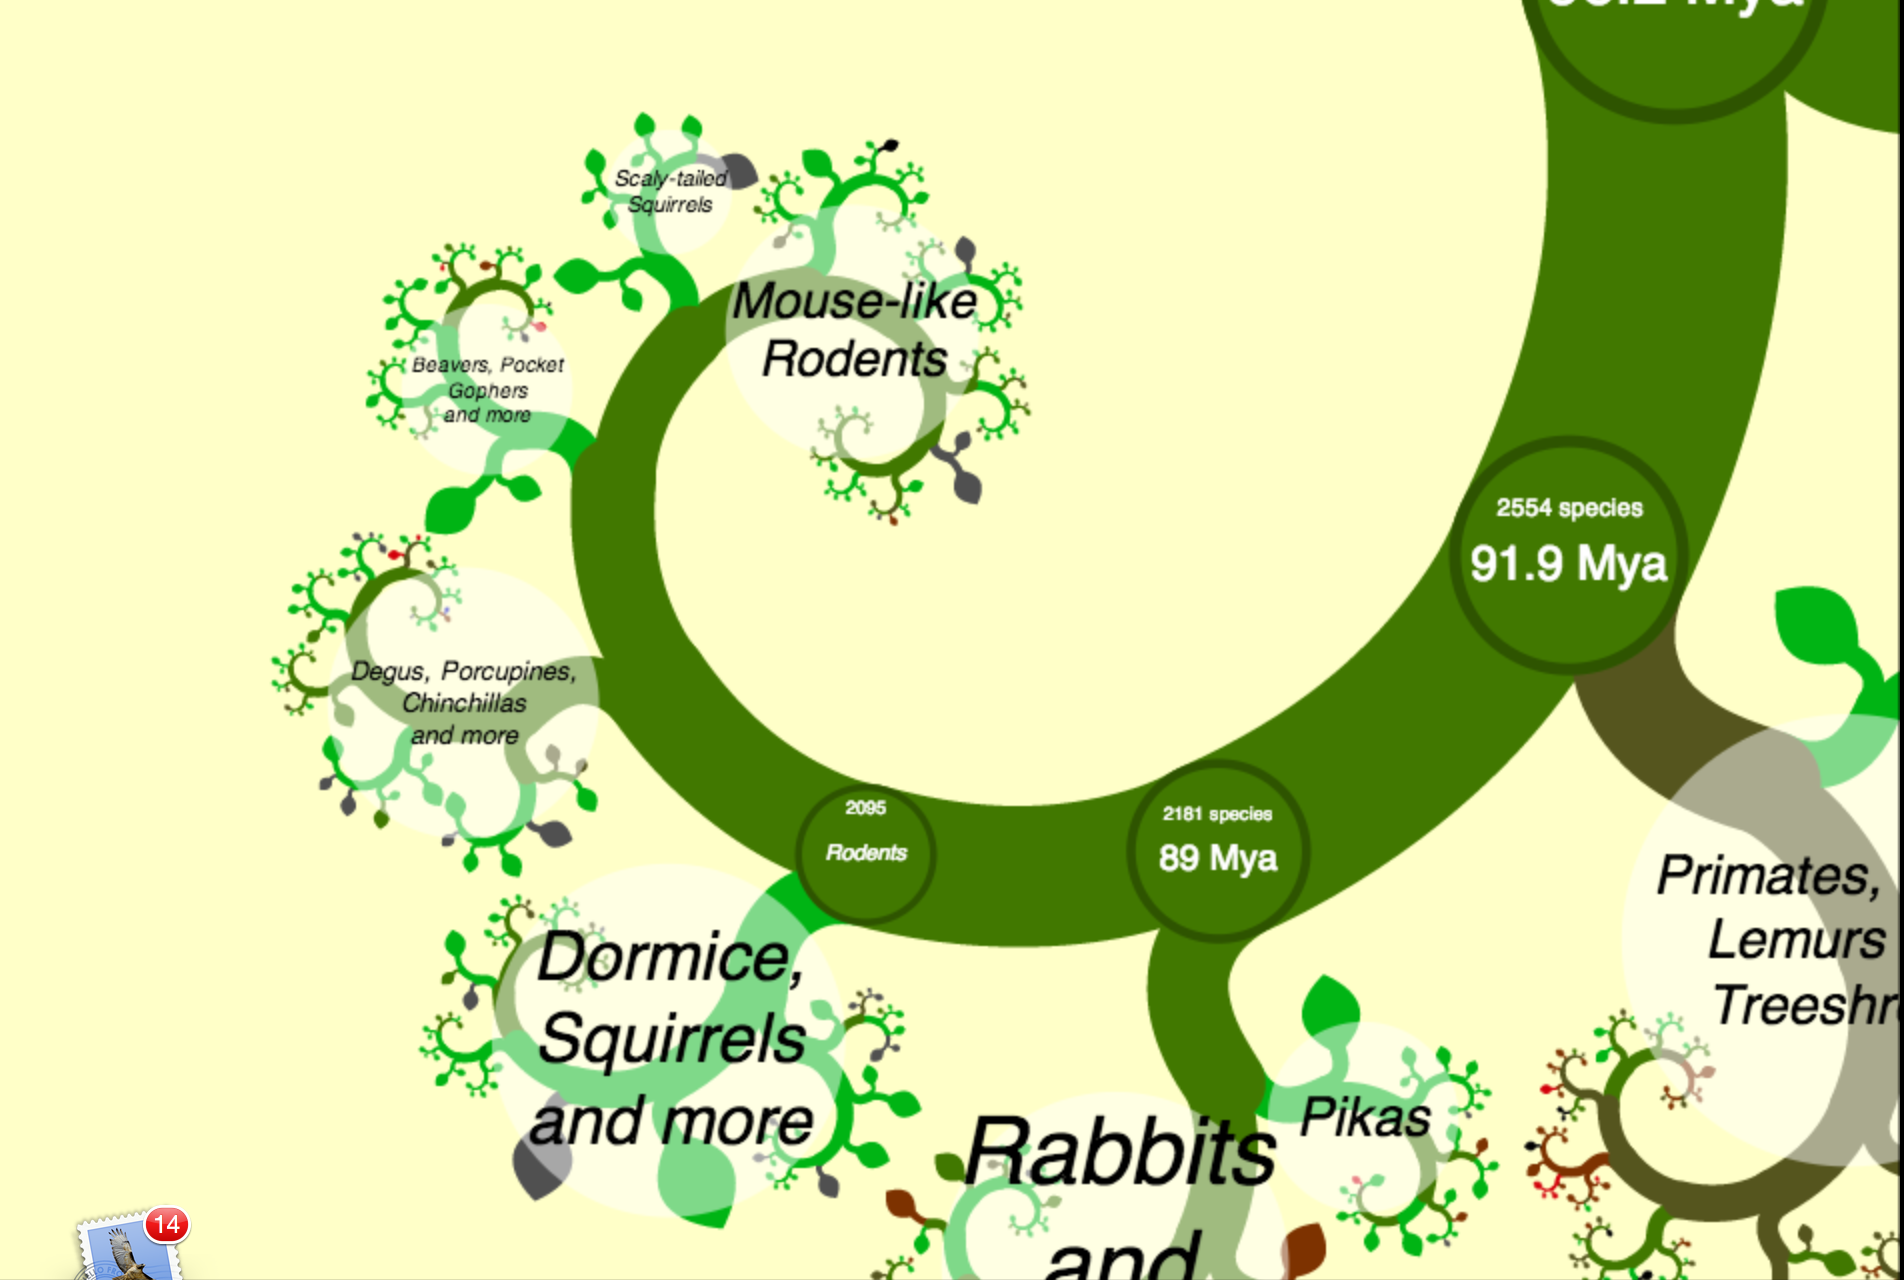
\includegraphics [width=15cm,height=8.8cm]{Rodent}
  \caption{Tree of Rodents: Zoom In to the Rodent Branch}
  \label{fig:rodent}
\end{figure}

\begin{figure}[H]
  \centering
  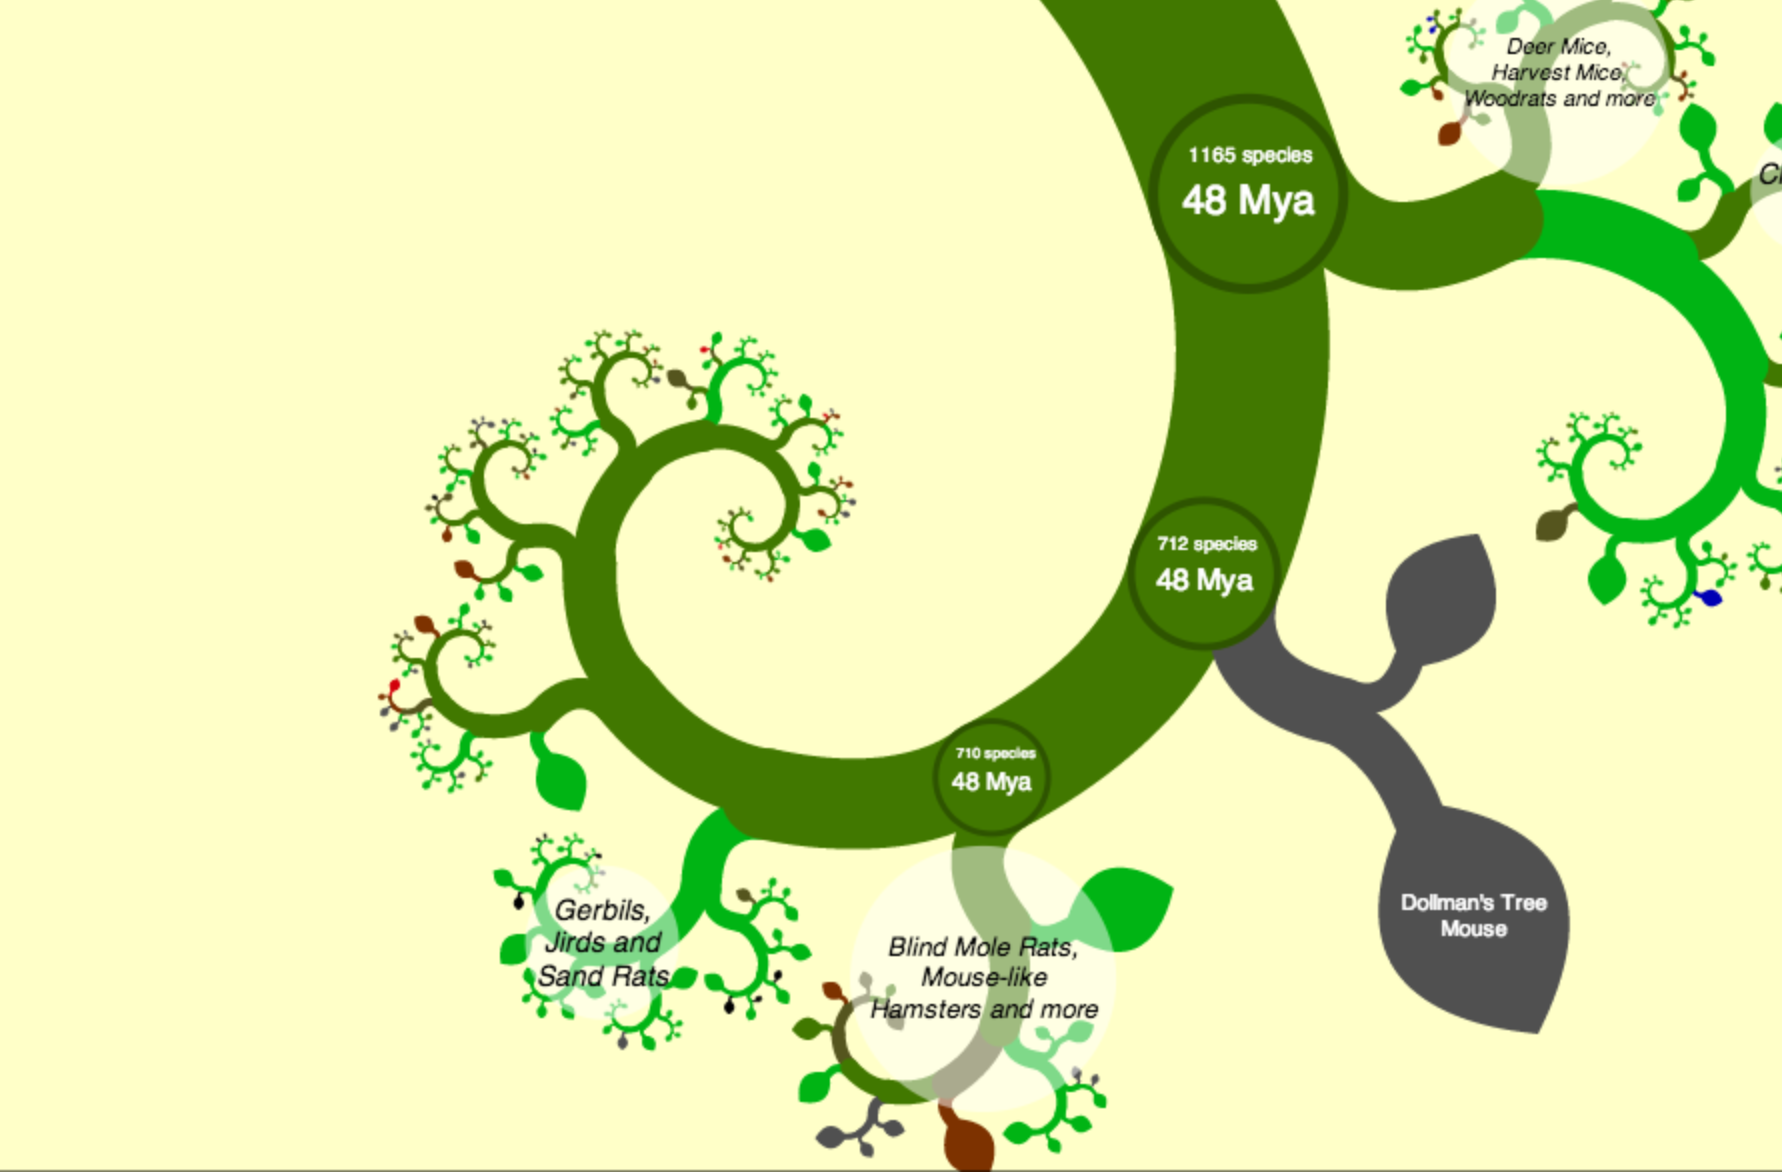
\includegraphics [width=15cm,height=8cm]{MouseLikeRodent}
  \caption{Zoom In the to Mouse Like Rodents Branch}
  \label{fig:mouseLikeRodent}
\end{figure}

\chapter{OneZoom Android Application Introduction}

This chapter will describe changes of implementation from the website software to android application. More details concerning how to improve the performance of the software and how to break the memory limitation for larger trees will be discussed in Chapter 4 and Chapter 5.

\section{ }


The website software use one class representing both link node and leaf node. Instead of using only one class, this application uses the original node class as a super class that takes charge of how to calculate positions of a node, how to get information of a node, and LeafNode, CircleNode(link node) as subclasses of the original class that take charge of how to draw themselves. Basically, the tree contains two type of nodes, one is the node with children nodes, the other is the node without any children. The nodes with children will create CircleNode objects, while the other ones will create LeafNode objects. 

\section{User Operation Listener}

The application now supports three kinds of user interaction: using one finger to drag the tree, double tap to zoom in, using two fingers two zoom in or zoom out. Drag and double tap are detected by inheriting GestureDetector.SimpleOnGestureListener class, while using two finger to zoom is detected by inheriting to ScaleGestureDetector.SimpleOnScaleGestureListener class. Then in the subclasses of these listeners, onScroll, onDoubleTap and onScale methods are overrode such that it could call the tree to be recalculated and the view to be updated. 

\begin{lstlisting}
	// event when using two fingers to scale
	@Override
	public boolean onScale(ScaleGestureDetector detector) {
		scaleFactor = detector.getScaleFactor();
		scaleFactor = Math.max(0.5f, Math.min(scaleFactor, 5.0f));
		drawview.zoomin(scaleFactor, detector.getFocusX(), detector.getFocusY());
		return true;
	}
	
	// event when scroll occurs
	@Override
	public boolean onScroll(MotionEvent e1, MotionEvent e2, float distanceX, float distanceY){
		drawview.drag(distanceX, distanceY);
		return true;
	}
	
	// event when double tap occurs    
	@Override
	public boolean onDoubleTap(MotionEvent e) {
		drawview.zoomin(e);
    		return true;
        }

\end{lstlisting}


\chapter{Memory handling issues}

\section{Problem description}

Memory is an important factor that needs to be considered under the circumstances of a quite large dataset and the relatively restricted resources of an Android.

As the dataset grows greater, the amount of memory needed for creating nodes also increases. By using chrome developer tools,  a snapshot of the heap memory usage can be obtained. For the mammals tree which has 5,020 species, there are 6.0 megabytes allocated in heap for creating these nodes. 12.2 megabytes and 29.1 megabytes are allocated for birds tree which has 9,993 species and for tetrapods tree which has 22,822 species respectively. The maximum dataset which represents all species contains about 2 million species. To build such a tree, the chrome browser needs to allocate approximate 2.4 gigabytes to 2.6 gigabytes, which is apparently not acceptable in most modern personal computers. The maximum amount of memory available for an android application is more limited than for a website software. More specifically, for each application running on Sumsang Galaxy S3, the maximum amount of memory available is 256 megabytes. This means the largest tree that can be built theoretically in the device has about 213,000 species, which is about one tenth the size of the complete tree of life.
\begin{table} [H]
	\centering % used for centering table
	\begin{tabular}{|c c c c|} % centered columns (4 columns)
		\hline %inserts double horizontal lines
		Tree Name & Richness  &  Total Heap Usage & Node Heap Usage\\% inserts table 
		%heading
		\hline  % inserts single horizontal line
		Mammals & 5020 &  8.3Mb & 6.0Mb\\  % inserting body of the table
		\hline
		Birds & 9993 &  14.4Mb & 12.2Mb\\
		\hline
		Tetrapods & 22822 & 34.1Mb & 29.1Mb\\ 
		\hline %inserts single line
		Bacteria & 408135 & N/A & N/A \\ [1ex] % [1ex] adds vertical space
		\hline
	\end{tabular}
	\label{table:nonlin} % is used to refer this table in the text
	\caption{Heap usage of tree with different amount of species in Chrome} % title of Table
\end{table}


Not only heap memory but also stack memory will increase as the number of species grows. When initialization begins, the website software creates the tree from the root. Then it recursively creates its children if the node is not a leaf node. The parameters which passed down to create its children are the dataset of the children, which is a string containing all metadata of its direct children and all further children. Therefore, for a leaf node which has a depth of n, its metadata will be copied in stack for n times during initialization. The greater amount of species a tree contains, the deeper its average depth will be. For the most balanced binary tree which contains N species, the average depth K of the tree should be:

\begin{equation*}
log_2 N + 1 < K < log_2 N + 2
\end{equation*}

In the worst case, where the binary tree is totally unbalanced, the average depth K of the tree should be:

 \begin{equation*}
	K = N/2
\end{equation*}

Take the largest tree released on the website tetrapods as an example. The data size of the tree is 1.5 megabytes. In the best case when the tree is well balanced, the average depth of the tree is about 16. Thus each metadata representing one species will be pushed into stack for 16 times in average. Therefore, the stack memory is expected to increase by at least 24 megabytes.

 The largest dataset that can currently be obtained is the bacteria tree. The data size of the tree is about 11 megabytes, while the total species of the tree is 408,135. Hence in the best case, the average depth of the tree will be 20. This multiplying the size of the dataset is the memory that will be allocated during initialization: 220 megabytes. The bacteria tree currently could not be loaded using chrome because running the software will exceed its maximum stack space. 
 
 Below are two tables gives comparison of total memory usage between different browsers and total memory usage right after initialization and a long time after initialization.
 
 \begin{table} [H]
	\centering % used for centering table
	\begin{tabular}{|c c c c|} % centered columns (4 columns)
		\hline %inserts double horizontal lines
		Tree Name & Richness  & Chrome & Firefox\\ % inserts table 
		%heading
		\hline  % inserts single horizontal line
		Mammals & 5020 &  53.1Mb & 10.39Mb\\  % inserting body of the table
		\hline
		Birds & 9993 &  58.5Mb & 20.00Mb\\
		\hline
		Tetrapods & 22822 & 80.7Mb & 45.6Mb\\ 
		\hline %inserts single line
		Bacteria & 408135 & N/A & 340.0Mb \\ [1ex] % [1ex] adds vertical space
		\hline
	\end{tabular}
	\label{table:nonlin} % is used to refer this table in the text
	\caption{Memory usage of different trees between Chrome and Firefox} % title of Table
\end{table}

\begin{table} [H]
	\centering % used for centering table
	\begin{tabular}{|c c c c|} % centered columns (4 columns)
		\hline %inserts double horizontal lines
		Tree Name & Richness  & Right after Initialization & Long time after initialization\\ % inserts table 
		%heading
		\hline  % inserts single horizontal line
		Mammals & 5020 &  53.1Mb & 93.3Mb\\  % inserting body of the table
		\hline
		Birds & 9993 &  58.5Mb & 111Mb\\
		\hline
		Tetrapods & 22822 & 80.7Mb & 148Mb\\  [1ex] % [1ex] adds vertical space
		\hline
	\end{tabular}
	\label{table:nonlin} % is used to refer this table in the text
	\caption{Memory usage of different trees between right after initialization and a long time after 
	initialization in Chrome } % title of Table
\end{table}


\section{Overview of the solution}

The solution of the issue is to dynamically add and delete nodes. As mentioned in the introduction of the software, only when a node is inside the display area and when the size of the node is big enough to be seen, the node will be drawn. The approach this application takes is to select the nodes whose larger bounding box(containing the node itself and all of its children) is inside the screen and the size of the which is greater than the visible threshold. Therefore, only parts of the tree will be built. Then when the user interacts with the view, the application will allocate memory to the nodes that should be built and deallocate memory from the nodes that are not visible.

When the application starts or when the user interacts with view, the application begins to test what nodes should be drawn. It starts from creating the root node. Then it tests whether the root node should be drawn based on two criteria: whether its larger bounding box is inside the screen and whether its size is greater than the drawing threshold. If the node satisfies the conditions, then its children should be built and tested using the same criteria. The nodes that satisfy the criteria will recursively create its children and test them until their children does not satisfy the test conditions or they don't have further children. 

\begin{figure} [H]
\begin{tikzpicture}[node distance = 5.5cm, auto]
    % Place nodes
    \node [block] (child1) {node = child1};
    \node [decision, right of=child1, node distance = 5.5cm] (test2) {$size > threshold$};
    \node [block, right of=test2, node distance = 5.5cm] (child2) {node = child2};
    \node [decision, above of=test2, node distance = 3.9cm] (test1) {inside screen};
    \node [block, above of=test1, node distance = 3.5cm] (build) {build node};
    \node [block, above of=build, node distance = 3cm] (root) {node = root};
    %Draw edges
    \path [line] (root) -- (build);
    \path [line] (build) -- (test1);
    \path [line] (test1) -- node[red]{Yes}(test2);
    \path [line] (test2) -- node[red]{Yes}(child1);
    \path [line] (test2) -- node[red]{Yes}(child2);
    \path [line] (child1) |- (build);
    \path [line] (child2) |- (build);
\end{tikzpicture}
\caption{Work flow of building part of the tree}
\end{figure}

Suppose the screen area is the yellow box in Figure~\ref{fig:screenAndBounding1}. The blue box is the larger bounding box of the root. It represents the boundary of the root node and of all of its children. Apparently, the root node is inside the screen and its size is big enough to be displayed. Therefore both children nodes should be created and tested continuously.

\begin{figure}[H]
  \centering
  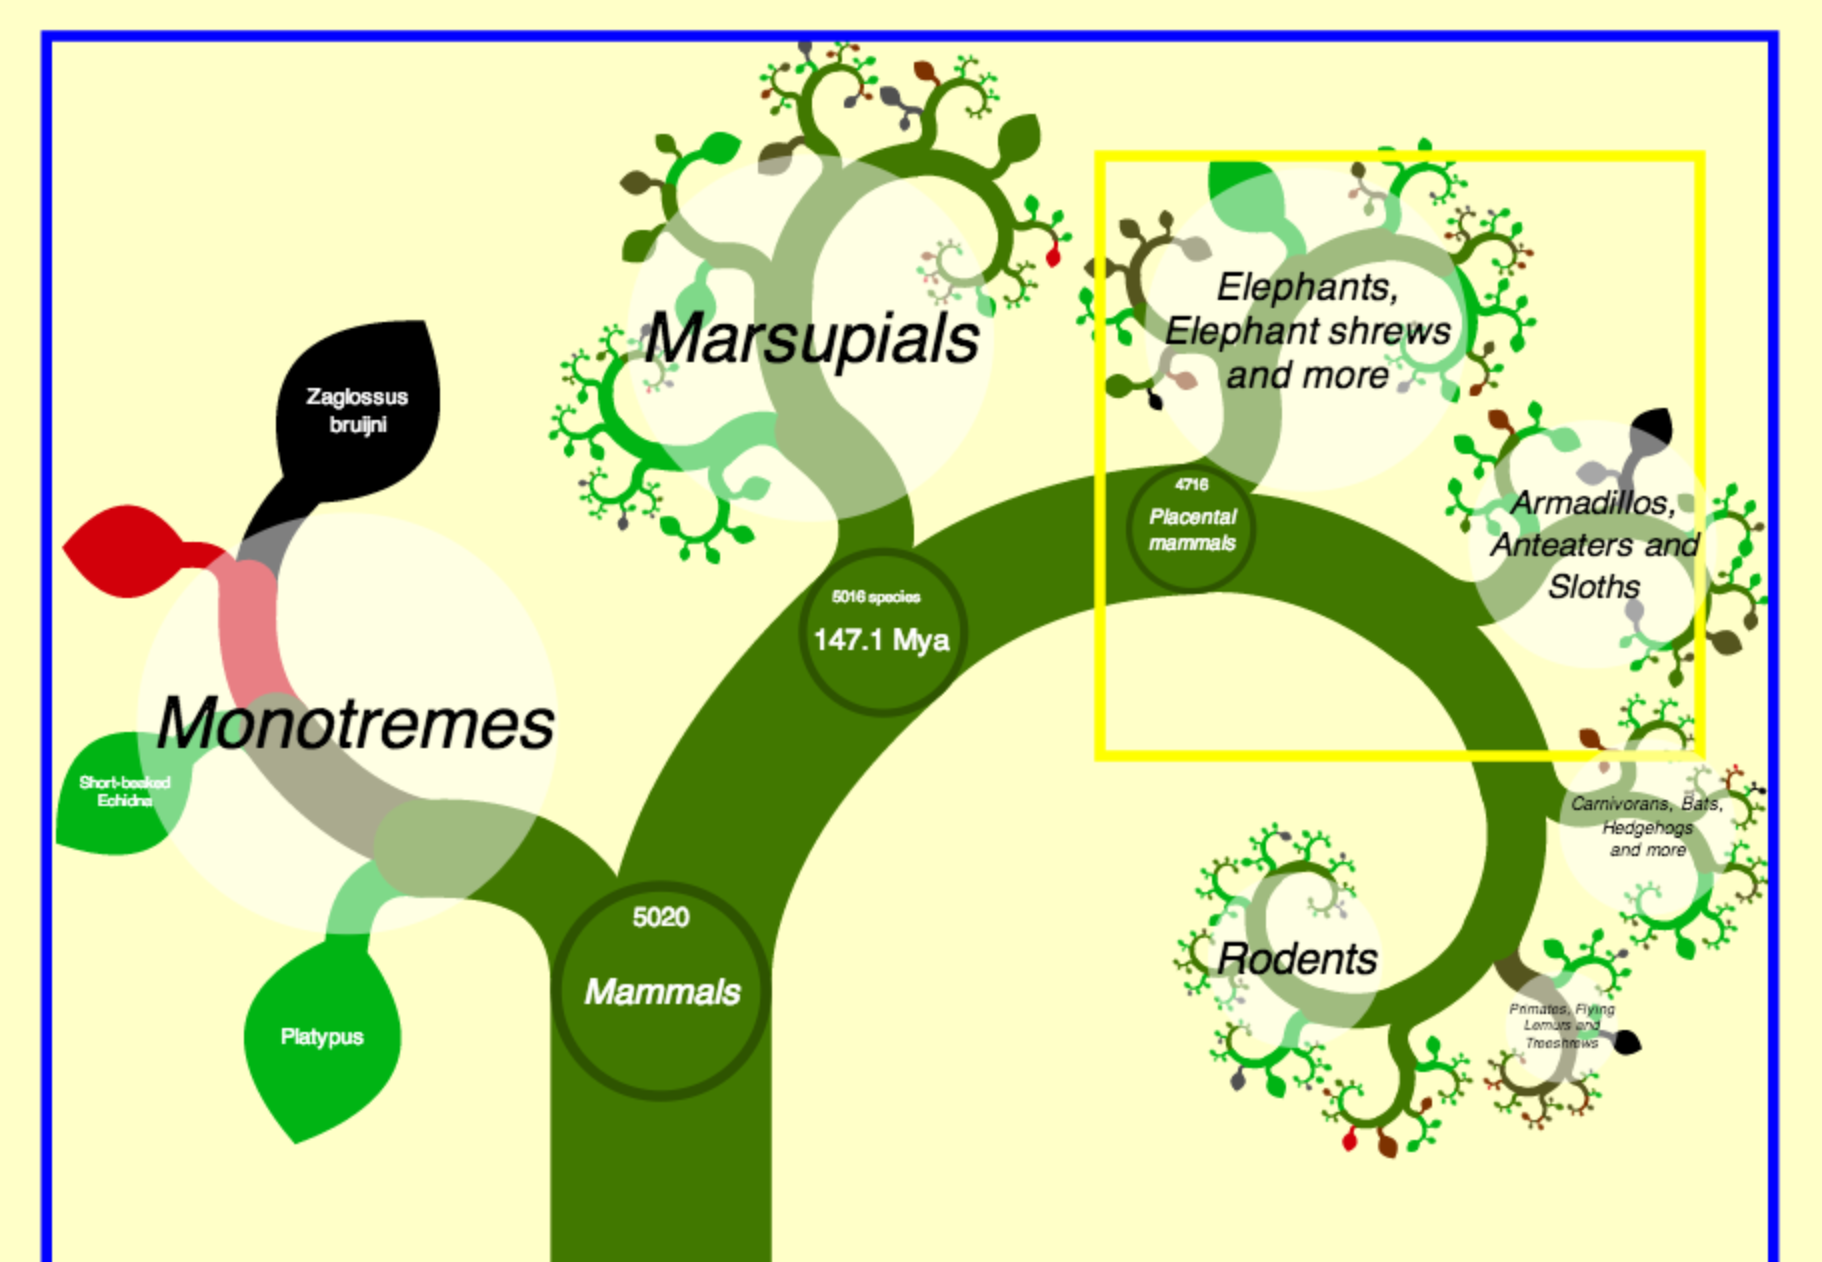
\includegraphics [width=15cm,height=8.8cm]{ScreenAndBounding1}
  \caption{Using Bouding Box to select branch}
  \label{fig:screenAndBounding1}
\end{figure}

In Figure~\ref{fig:screenAndBounding2}, the bounding box of child1(blue box) is out of the screen, while that of child2(red box) is still in the screen(Here it is assumed that all children on the left hand side are child1). Therefore, the application will continue to build the children of child2 and test them. In contrast, the children of child1 will not be further checked. 

\begin{figure}[H]
  \centering
  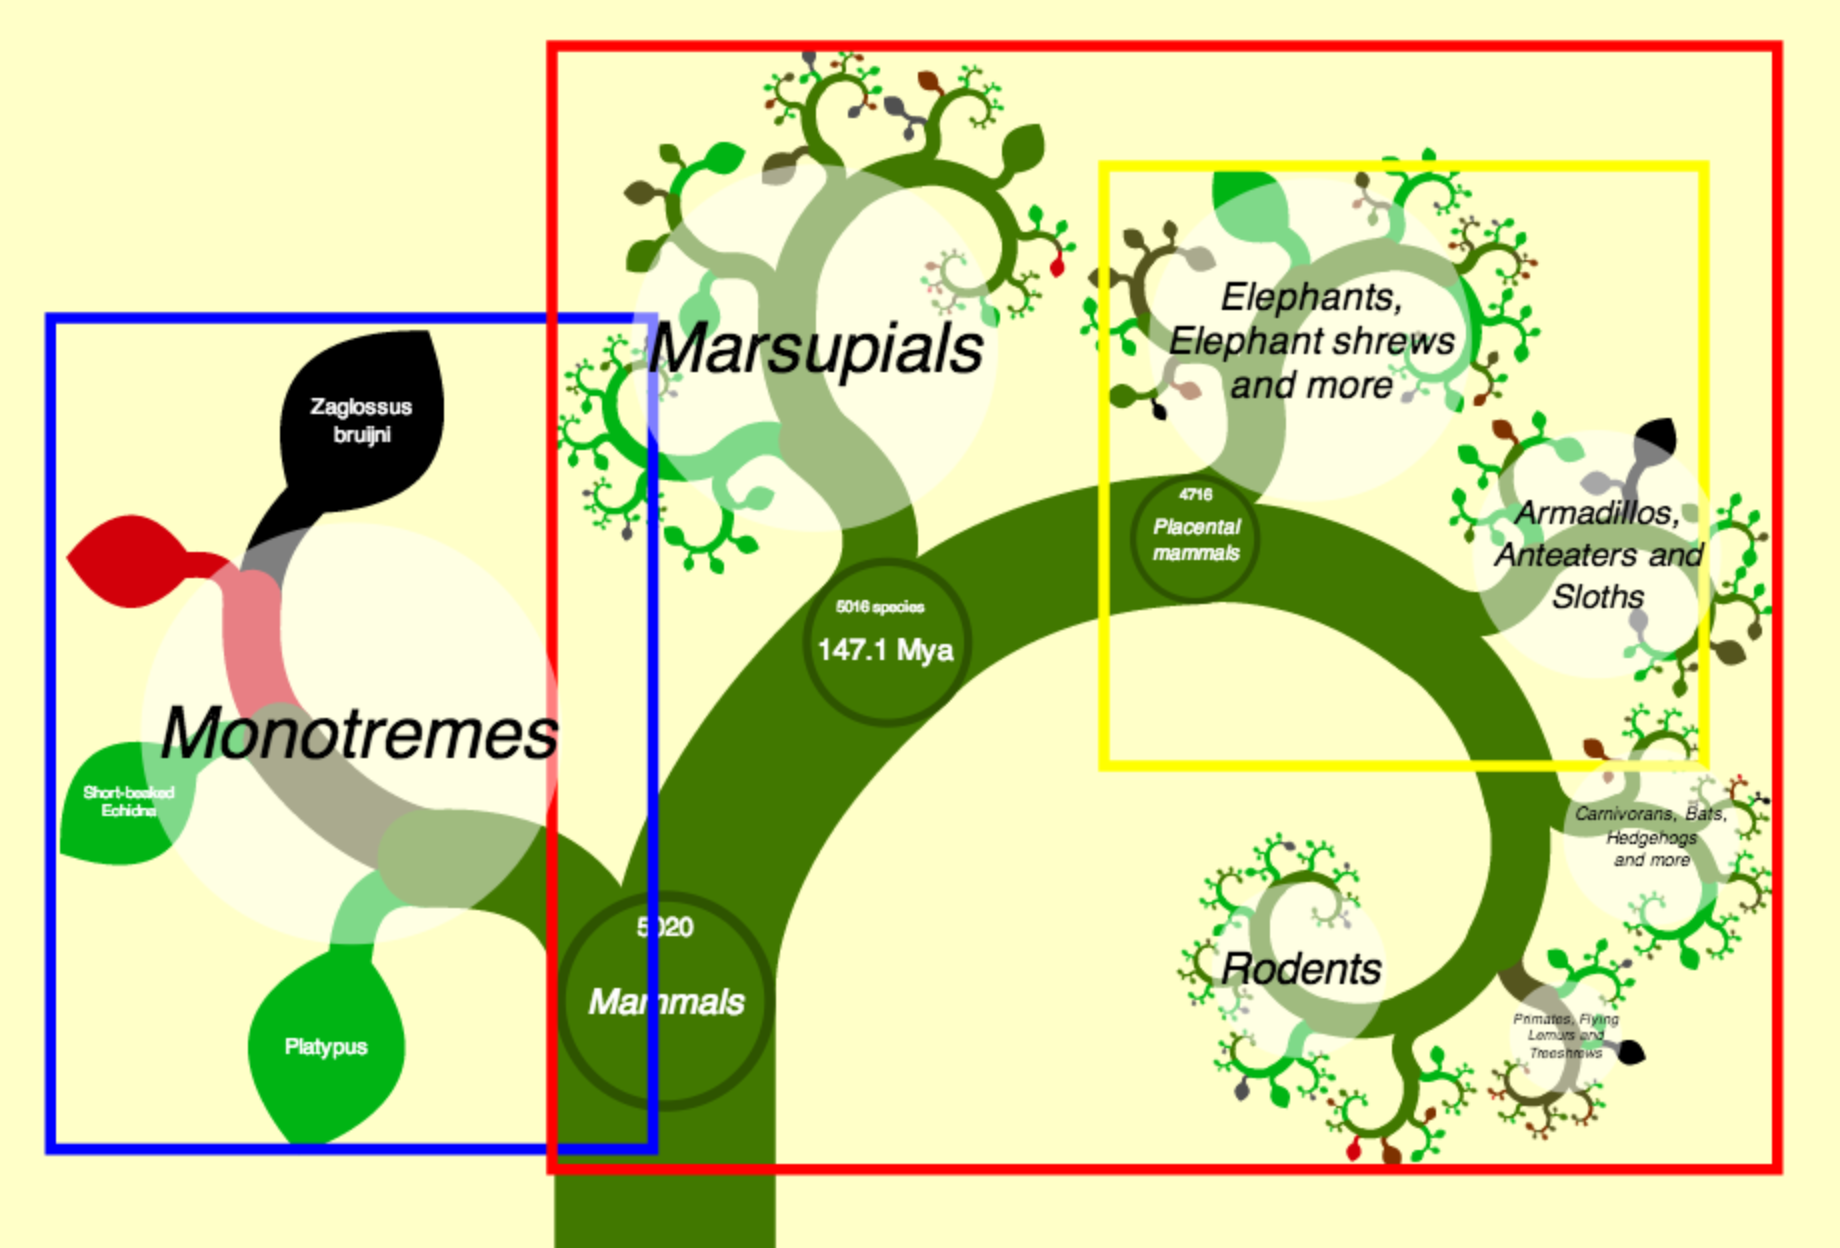
\includegraphics [width=15cm,height=8.8cm]{ScreenAndBounding2}
  \caption{Bounding box of child1 and child2 of root}
  \label{fig:screenAndBounding2}
\end{figure}

Further building will be continued until reaching the leaf node or the node is out of the screen or the node is too small to be displayed.



\section{Creating a new data format}

Since only part of the tree would be built, the information of the nodes that relies on its children, like richness, age, could not be calculated by using the raw data. Hence, a new dataset containing this information needs to be built. For example, the dataset discussed in Chapter 2: 

\begin{center}
	((A:1.5,B:1.5)C:2,D:3.5)E
\end{center}

should be changed as:

\begin{center}
	((A[1\_0],B[1\_0])C[2\_1.5]:1,D[1\_0])E[3\_3.5]
\end{center}

Inside the square bracket, the first number represents the richness of a node and the second number represents the age of a node.

Except for the richness and age, the calculation of outer bounding box also relies on its children. Therefore, the bounding box is also expected to be appended in the raw data. However, in order to avoid the raw data becoming too long and too complex, a database is created to record those information. It also contains other information like the ratio of a node, the x position and y position relative to the root of the tree. Such data is used to test whether the node should be drawn. 

The database also includes the id of both children. When the node pass the test, then it can build and test its children according to their id. In order to build a node, data of it need to be accessed. Instead of storing the whole data string into the database, the application records the start and end position of the node in the data string. What's more, as the data for the children can also be accessed by referring to the start and the end position in the database, the application does not need to pass down the whole data string as parameters. Instead, the application creates new nodes by passing down the children id. Therefore, each substring which represents a node in the raw data will be created only once, which greatly reduce the use of stack memory. 

\begin{figure}[H]
  \centering
  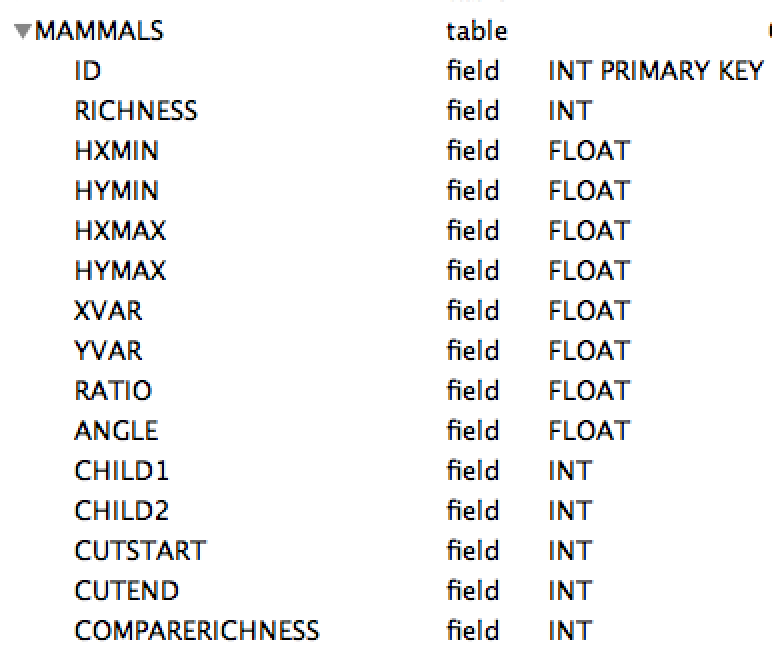
\includegraphics [width=15cm,height=7.8cm]{Database}
  \caption{Database columns}
  \label{fig:mammal}
\end{figure}

Again, because of memory size limitation, the application can't build a database containing all nodes. Instead, only for the nodes whose richness or whose parent richness is greater or equal to a threshold, the node information will be recorded in the database. For the nodes whose richness is smaller than the threshold, the start and end position of its data will represent itself plus both of its children. For the bacteria tree, the threshold is 500. The table of bacteria contains  19543 rows, which is about 2.5\% the total amount of nodes in the original bacteria raw data. For the rest trees, the threshold is 50.

In the following paragraph, the node in the database whose richness value is smaller than threshold will be called mini root node. When this node passes the test of displaying, the application will not continue build and test because it does not have enough information about its children. Instead, the application will continue building all of children directly from string. 

\section{Dynamic adding and deleting of nodes}

This section gives more details about how the application adds and deletes nodes. Running list and non initialization list are used during the process of adding and deleting nodes.

When the application starts, it builds the root node and adds it into non initialization list. The running list is initialized as an empty list. Then each time user interacts with the view, the recalculation begins.

The recalculation begins from the root node. The first step is to test the node position, size and its richness. There are four types of possible test results. Test result 0 means the node should not be drawn. Test result 1 means the node should be drawn and its a leaf node. Test result 2 and test result 3 means the node should be drawn and they are link nodes. The difference is that test result 3 means the richness of the node is smaller than the threshold, thus it's a mini root node. 

If the test result is 0, the recalculation should stop here. Otherwise if the result is not 0 and if the node is not in the running list, the node will be added into the running list. Specifically, if the result is 1, the recalculation will also end, while if the result is 3, all children of the mini root node will be built and no further check is needed. If the test result is 2, the children of this node will be built by referring to records from the database and the steps mentioned above will be repeated.

\begin{figure} [H]
\begin{tikzpicture}[node distance = 5.5cm, auto]
    % Place nodes
    \node [block] (children) {node = child1 node = child2};
    \node [decision, right of=children, node distance = 5.5cm] (threshold) {$richness < threshold$};
    \node [block, right of=threshold, node distance = 5.5cm] (build) {Build all children of mini root};
    \node [decision, above of=threshold, node distance = 3.3cm] (leaf) {$richness=1$};
    \node [block, above of=leaf, node distance = 3cm] (add) {add node to running list};
    \node [block, above of=add, node distance = 2.5cm] (remove) {remove node from non initialization list};
    \node [decision, above of=remove, node distance = 3cm] (test) {display node?};
    \node [block, above of=test, node distance = 3cm] (root) {node = root};
    \node [decision, right of=test, node distance = 5.5cm] (inRunning) {node in running list?};
    \node [block, below of=inRunning, node distance = 3.5cm] (add2) {add node to non initialization list}; 
    \node [block, right of=leaf, node distance = 5.5cm] (end2) {end};


    %Draw edges
    \path [line] (root) -- (test);
    \path [line] (test) -- node[red]{Yes}(remove);
    \path [line] (test) -- (remove);
    \path [line] (remove) -- (add);
    \path [line] (add) -- (leaf);
    \path [line] (leaf) -- node[red]{No}(threshold);
    \path [line] (threshold) -- node[red]{Yes}(build);
    \path [line] (threshold) -- node[red]{No}(children);
    \path [line] (children) |- (test);
    \path [line] (test) -- node[red]{No}(inRunning);
   \path [line] (inRunning) -- node[red]{No}(add2);
    \path [line] (leaf) -- node[red]{Yes}(end2);

\end{tikzpicture}
\caption{Work flow of adding nodes on the tree}
\end{figure}

From the picture we can see that when the node is in the running list and it should not be displayed, the node and its children will not be removed and not deallocated in the running list. This is due to performance consideration. Logically, the non initialization list represents the nodes whose children are not built. If the node is moved from running list to non initialization list, then all of its children also need to be removed from running list and get deallocated. However, these nodes are possible being needed to be built again in further user interaction, which will cost great amount of time. Therefore, by remaining nodes in running list, the application could save time from deallocating nodes as well as allocating nodes. 

As the user does more and more interaction, the remaining memory might be not enough for allocating new nodes. Therefore, after adding new nodes is done, the application will check whether there are enough space left(10 megabytes in the current application). If the memory is not enough, then deleting will start.

The first step of deleting is to test the possibility of the nodes in the running list being displayed in the following user interactions. The nodes that should be displayed will be assigned to the maximum value of Integer in java. In general, the closer the node's bounding box is to the screen and the bigger the node's size is, the higher possibility the node will be assigned. Suppose that d is the distance between bounding box and screen, s is the size of nodes, T is the visible threshold, WH is the average of the width and height of the screen. Then the possibility of the node is:

\begin{center}
$Possibility = Integer.Maximum - P(d) - P(s) (d \textgreater 0, s\textless T)$

$P(d) = 0.6*x^2 - 0.1*x$

$P(s) = 0.6*x^2 - 1.1*x + 0.5$
\end{center}

Figures like 0.6, -0.1, -1.1 are not calculated by accurate mathematical model. The formulas are generated from points like (0,0), (0.5,0.1), (1,0.5) in P(d) and (0,0.5), (0.25,0.2), (1,0) in P(s). The reason for selecting these points are to ensure the value of possibility fluctuates between 0 and 1 and the speed of the change should be bigger when distance is far and when size is small.

\begin{figure}[H]
				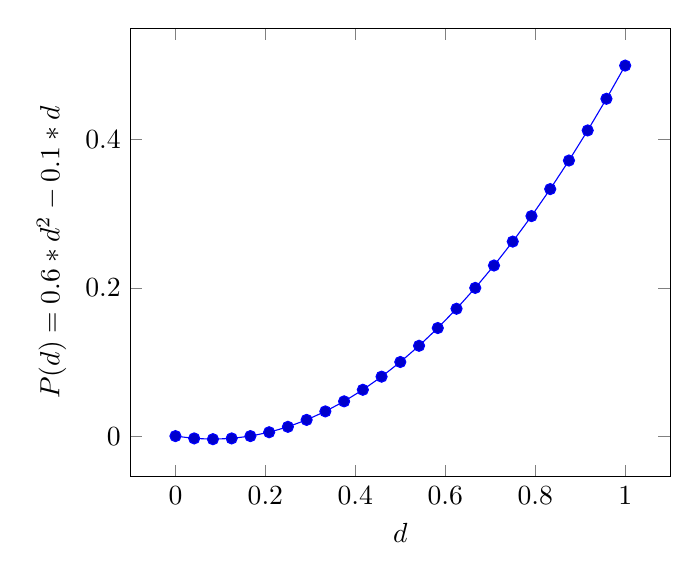
\begin{tikzpicture}
 				 \begin{axis}[ 
				    xlabel=$d$,
 				   ylabel={$P(d) = 0.6*d^2 -0.1*d $}
					  ] 
 				   \addplot+[domain = 0:1]
   				  {0.6*x^2 - 0.1*x}; 
 				 \end{axis}
				\end{tikzpicture}
        \caption{Possibility with distance}\label{fig:animals}
\end{figure}

\begin{figure}[H]
				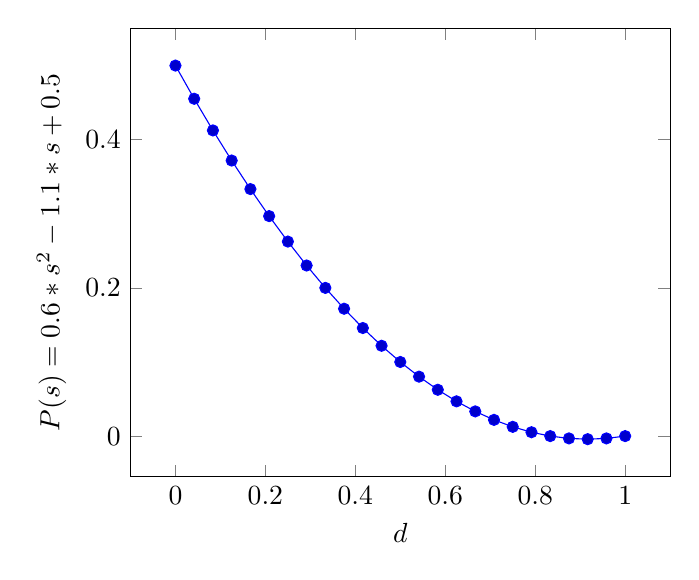
\begin{tikzpicture}
 				 \begin{axis}[ 
				    xlabel=$d$,
 				   ylabel={$P(s) = 0.6*s^2 -1.1*s + 0.5 $}
					  ] 
 				   \addplot+[domain = 0:1]
   				  {0.6*x^2 - 1.1*x +0.5}; 
 				 \end{axis}
				\end{tikzpicture}
        \caption{Possibility with size}\label{fig:animals}
\end{figure}

After calculating the possibility of nodes in running list, the running list will be sorted according to the nodes possibility. Then remove the first node as well as all of its children from the running list and free the memory of these nodes. Then continue to remove the node from the beginning of the running list until there are enough unused memory for this application.

\begin{figure} [H]
\begin{tikzpicture}[node distance = 5.5cm, auto]
    % Place nodes
    \node [block] (recalculation) {Recalculation};
    \node [block, right of=recalculation, node distance = 5.5cm] (poss) {Calculate Possibility};
    \node [block, right of=poss, node distance = 5.5cm] (sort) {Sort running list};
    \node [decision, below of=sort, node distance = 2.7cm] (space) {$memory < 10 Mb$};
    \node [block, left of=space, node distance = 5.5cm] (remove) {Remove 1st node \& its children from running list};    
    %Draw edges
    \path [line] (recalculation) -- (poss);
    \path [line] (poss) -- (sort);
    \path [line] (sort) -- (space);
	\draw [->] (7.2,-2.4) -- (9.9,-2.4);
	\draw [->] (9.9,-3.0) -- (7.2,-3.0);
\end{tikzpicture}
\caption{Work flow of deleting nodes on the tree}
\end{figure}

\subsection{Result}

While the application is running, the memory usage of the application is expected to increase as thread will initialize nodes during its idle time. More details can be seen in next chapter. The table below gives comparison of memory usage before and after optimization when the application starts.

\begin{table} [H]
	\centering % used for centering table
	\begin{tabular}{|c c c c|} % centered columns (4 columns)
		\hline %inserts double horizontal lines
		Tree Name & Richness  & Before & After\\ % inserts table 
		%heading
		\hline  % inserts single horizontal line
		Mammals & 5020 & 89Mb   & 86Mb\\  % inserting body of the table
		\hline
		Birds & 9993 &  95Mb & 86Mb\\
		\hline
		Tetrapods & 22822 & 104Mb & 86Mb\\ 
		\hline %inserts single line
		Bacteria & 408135 & N/A & 89Mb \\ [1ex] % [1ex] adds vertical space
		\hline
	\end{tabular}
	\label{table:nonlin} % is used to refer this table in the text
	\caption{Comparison of memory usage before and after optimization} % title of Table
\end{table}

The memory usage of the tree of mammals, birds and tetrapods are bigger than that in Chrome or Firefox because the application creates an object containing all raw data, a database and two bitmap used for solving performance issues, while all these are not used in the website software.

The memory usage after optimization is almost not changed with the increase of richness of the tree. For the bacteria tree, the richness threshold is higher than that of other trees. Therefore, it is more likely to reach a mini root node and initialize all of its children during initialization. Hence, it has a higher memory usage than other trees.

\chapter{Performance Issues}

Two problems greatly affect the performance of this application. One is over long loading time, the other is slow user interaction response time. Both of the problems are largely influenced by the processing capacity of a mobile phone processor as well as the size of the dataset. 

\section{Loading Time}

Before the phylogenetic tree first gets drawn, the application needs to load data from a string and create objects for the logical units in it, which represents a species or a group of some species. Then pre calculation which involves all the nodes on the tree gets called in order to calculate the relative position of each node. Both the cost of loading data and the cost of pre calculation is linear. Hence, the loading time of a phylogenies tree is expected to increase linearly with the size of the data. By using an older version of the application, we can test the loading time of different phylogenetic trees on a Sumsang Galaxy S3 device. When loading the mammal tree which has 5,020 species, the loading time is 1,761 millisecond, while loading the bird tree which has 9,993 species and tetrapods tree which has 22,822 species, the loading time increases to 3,683 milliseconds and 8,177 milliseconds respectively. The increase of loading time with the increase of species can also be observed in the website software. More details could be seen in the table below. As the ambition of this project is to build a tree of all existing and existed species, which has approximate 2 million species, the loading time of that tree could be intolerable.

\begin{table} [H]
	\centering % used for centering table
	\begin{tabular}{|c c c c c c|} % centered columns (4 columns)
		\hline %inserts double horizontal lines
		Tree Name & Richness  & Android & Chrome & Firefox & Safari\\% inserts table 
		%heading
		\hline  % inserts single horizontal line
		Mammals & 5020 & 1761ms & 319ms & 239ms & 501ms \\  % inserting body of the table
		\hline
		Birds & 9993 & 3683ms & 660ms & 538ms & 1452ms \\
		\hline
		Tetrapods & 22822 & 8177ms & 1951ms & 1087ms & 2972ms\\ 
		\hline %inserts single line
		Bacteria & 408135 & N/A & N/A & 17016ms  & 59684ms\\ [1ex] % [1ex] adds vertical space
		\hline
	\end{tabular}
	\label{table:nonlin} % is used to refer this table in the text
	\caption{Loading Time on Android and website version before memory and performance optimizing} % title of Table
\end{table}

In order to shorten the loading time, several bitmaps of different trees are stored as resources. When a user selects one of the tree, the corresponding bitmap would be drawn on canvas. In the meantime, another thread would be created to load data and do pre calculation. The main UI thread and the calculation thread share a flag by which the view object knows whether the pre calculation is done or not. When the pre calculation is on progress and the user drags or zooms on the tree, the view object will use the built in method of canvas class to scale or translate the stored bitmap. When pre calculation is finished, the calculation thread would send a message to the main UI thread so that it will invalidate the view by draw nodes.

Essentially, in the previous design, users spend time waiting for the data to be loaded and calculated. In the later design, the tree is drawn using bitmap even before the tree is created. Therefore, from a user perspective, the loading time of any tree could be reduced to unnoticeable. 

\begin{table} [H]
	\centering % used for centering table
	\begin{tabular}{|c c c c|} % centered columns (4 columns)
		\hline %inserts double horizontal lines
		Tree Name & Richness  & No optimization  & After optimization \\% inserts table 
		%heading
		\hline  % inserts single horizontal line
		Mammals & 5020 & 1761ms & 398ms   \\  % inserting body of the table
		\hline
		Birds & 9993 & 3683ms & 393ms  \\
		\hline
		Tetrapods & 22822 & 8177ms & 405ms   \\ 
		\hline %inserts single line
		Bacteria & 408135 & N/A & 380ms  \\ [1ex] % [1ex] adds vertical space
		\hline
	\end{tabular}
	\label{table:loadingCamparison} % is used to refer this table in the text
	\caption{Result of loading time after optimizing in Android} % title of Table
\end{table}

From Table ~\ref{table:loadingCamparison} we can see that the cost of loading time is much smaller than that before optimization. Besides, the increase of the size of tree doesn't affect the length of loading time any more.

\section{User Interaction}

Another factor that could affect user experience is the slow response time for user interaction. 
When user drags or zooms on the view, the view listener would receive a set of drag or zoom messages. For each message it receives, the application is supposed to recalculate which nodes should be display and create and add those nodes which has not been created yet into the drawing array. Then it will call the view to update itself. Since both the speed of recalculating and the speed of redrawing nodes are much more slower than the speed of generating drag or zoom messages, user could feel great delay waiting for these two procedures finishing.


\begin{figure}[H]
\begin{tikzpicture}[node distance = 6cm, auto]
    % Place nodes
    \node [block] (view) {View};
    \node [block, right of=view] (operation) {Drag or Zoom};
    \node [block, below of=operation, node distance = 3cm](recalculation) {Recalculate drawing nodes};
    \node [block, left of=recalculation] (update) {Draw nodes};
    %Draw edges
    \path [line] (view) -- node[red]{Listen}(operation);
    \path [line] (operation) -- (recalculation);
    \path [line] (recalculation) -- (update);
    \path [line] (update) -- (view);
\end{tikzpicture}
\caption{Previous working flow of main UI thread}
\end{figure}

\subsection{Using thread and message queue to discard extra mouse move message}

In order to reduce the response time, the extra finger move messages should be discarded. Another thread and message queue is used to solve this problem. When a user triggers a set of move actions, a set of recalculation messages will be sent from the main UI thread to the calculation thread. In the calculation thread, when it catches a recalculation message while there are other recalculation messages in the message queue, then the current recalculation message will be discarded. Otherwise, the recalculation method will be called. Hence, when there are several recalculation messages being sent, only the last one will be processed. When the recalculation is over, the calculation thread will send message to invalidate the view. 

 \begin{figure}[H]
 \begin{tikzpicture}[node distance = 5.5cm, auto]
    % Place nodes
    \node [block] (view) {View};
    \node [block, right of=view] (operation) {Drag or Zoom};
    \node [block, below of=operation, node distance=3cm] (looper) {Looper};
    \node [block, below of=looper, node distance = 3cm] (handler) {Handler};
    \node [block, right of=looper, node distance = 5.5cm] (catcher) {Catch next message};
    \node [decision, below of=handler, node distance = 3.5cm] (decision) {The only recalc message?};
    \node [block, left of=decision] (recalculation) {Recalculation};
    %Draw edges
    \path [line] (view) -- (operation);
    \path [line] (operation) -- node[red] {Send Message} (looper);
    \path [line] (looper) -- (handler);
    \path [line] (handler) -- (decision);
    \path [line] (decision) -| node[red, near end]{Yes}(catcher);
    \path [line] (catcher) -- (looper);
    \path [line] (decision) -- node[red]{No}(recalculation);
    \path [line] (recalculation) -- node[red]{Update View}(view);
\end{tikzpicture}
\caption{How recalculation thread deals with message}
 \end{figure}
 
 \subsection{Using idle thread to prepare nodes}

The calculation thread is active when the user starts interacting with the view. The time users waiting for the view to draw nodes are decided by how long the thread would take to add new nodes. An improvement has been made by using the idle time of the calculation thread to allocate memories for the nodes that are likely being built in the following user interaction. 

Adding new nodes during idle time is very similar to deleting unused nodes. After adding new nodes, if there enough memory, the application will send message calling the calculation thread to calculate the possibility of the nodes in the non initialization list. It is followed by sorting these nodes according to their possibility. Then move the node from non initialization list to running list and check whether its richness is smaller than the richness threshold(500 for bacteria tree). If it is, then the node is a mini root so create all of its children, otherwise build its direct children and add both children to non initialization tree. 

This is one cycle of allocating new nodes during idle time. When the cycle ends, the thread will send another idle calculation message. If the thread does not have recalculation message and there are enough space, then the cycle will be gone through again and one more idle calculation message will be generated. Otherwise, the idle calculation will terminate and be reactive after next user interaction.

 \begin{figure}[H]
 \begin{tikzpicture}[node distance = 5.5cm, auto]
    % Place nodes
    \node [block] (term1) {Terminate};
    \node [block, below of=term1, node distance = 3.5cm](term2) {Terminate};
    \node [decision, right of=term1, node distance=5.5cm] (test) {Recalculation in Message Queue?};
    \node [decision, below of=test, node distance = 3.5cm] (test2) {Enough memory?};
    \node [block, right of=test2, node distance = 5.5cm] (sort) {Sort non initialization list};
    \node [block, above of=sort, node distance = 3.5cm] (build) {Initialize one node from non initialization list};    
    \node [block, above of=test, node distance =3.5cm] (poss) {Calc possibility in non initialization list};
    \node [block, above of=term1, node distance = 3.5cm] (recalc) {Recalculation Finish};
  
   
    %Draw edges
    \path [line] (test) -- node[red] {Yes}(term1);
    \path [line] (test2) -- node[red] {No}(term2);
    \path [line] (recalc) -- (poss);
    \path [line] (poss) -- node[red] {Send Message} (test);
    \path [line] (test) -- node[red] {No}(test2);
    \path [line] (test2) -- node[red]{Yes}(sort);
    \path [line] (sort) --(build);
    \path [line] (build) -- (test);

\end{tikzpicture}
\caption{Calculation during idle time}
 \end{figure}


\subsection{Using cached bitmap to update view before calculation is done}
 
 Though the number of calculation messages being processed would be reduced to a minimum number, users would still feel a bit of delay in refreshing the view since the view only gets updated after the recalculation is done, which may take a bit of time. Moreover, as only the last recalculation message in the message queue gets processed, the tree will be placed back to the position where the last mouse move message was triggered. This could result in inconsistent display. 
 
This problem is solved by using a cached bitmap to update the view. When the application observes a user operation, it will not only send a message to another thread, but also update the view. Then in the onDraw method of the view class, it would test whether the user is still interacting with the view and whether recalculation is over. If user's finger is off the screen and the recalculation is over, it will draw the tree objects, otherwise it will translate or scale the bitmap stored previously to give users a continuous display. The size of the bitmap is actually greater than the size of the screen. When the user drags or zooms out the view , the part that was out of the screen would be moved into the screen. If the bitmap is the same size as the screen, then user would see a compressed picture on the screen. 
When the recalculation is done, it will send message to update the view. From a user perspective, when he or she drag on the view, he or she would get a consistent display. However, if the user zooms in, he or she would get an unclear picture first, since scaling on bitmap is only scaling on pixels. However, a precise picture of the tree would replace the unclear one soon. 

\begin{figure}[H]
\begin{tikzpicture}[node distance = 4cm, auto]
    % Place nodes
    \node [block] (view) {View};
    \node [block, right of=view, node distance = 5.5cm] (operation) {Drag or Zoom};
    \node [block, right of=operation, node distance = 5.5cm] (update) {Update View};
    \node [block, above of=update, node distance = 3cm] (recalculation) {Recalculation};
    \node [decision, below of=update, node distance = 4cm] (test) {Test whether should use bitmap};
    \node [block, left of=test, node distance = 5.5cm] (bitmap) {Translate and Scale bitmap};
    \node [block, below of=test] (redraw) {Draw Using Node Object};
    \node [block, left of=redraw, node distance = 5.5cm] (store) {Cache New Bitmap};

   %Draw edges
    \path [line] (view) -- (operation);
    \path [line] (operation) |- node[red, near end, above]{Message to Another Thread}(recalculation);
    \path [line] (recalculation) -- node[red, left] {Message to Main UI} (update);
    \path [line] (operation) -- (update);
    \path [line] (update) -- (test);
    \path [line] (test) -- node[red, near end]{No}(redraw);
    \path [line] (redraw) -- (store);
    \path [line] (test) -- node[red]{Yes}(bitmap);
    \path [line] (store) -| (view);
    \path [line] (bitmap) -| (view);
 
\end{tikzpicture}
\caption{How to update view}
\end{figure}

\subsection{Test use bitmap or do actual drawing}

Both listening to user actions, drawing nodes, drawing bitmap are processed in main UI thread. Therefore, when the application is drawing bitmap or drawing nodes, the application is not listening to user interaction at the same time. The time spent on drawing bitmap is nearly 0 milliseconds, while the time spent on drawing nodes is fluctuate between 50 to 150 milliseconds. This means that there will be obvious delays if the view gets updated by drawing nodes while user is still interaction with the views.

Therefore, the application need to avoid drawing nodes during user interaction. This is done by set a flag named duringInteracion when  the view detects action down and reset the flag when the view detects action up, which suggests the user's finger is off the screen. 

There is one more thing needing to be tested for whether to use bitmap . When the processor of a mobile device is switched to handle recalculation message, it could quickly discard all but the last recalculation message and process it. However, while the recalculation is being done, user could continue operating on the mobile device. For example, the calculation thread may be switched while the user is moving his or her finger on the screen. As a result, when the calculation is done, the position of the tree object is not where the user's finger points to. If the user's finger is off the screen now, the application would draw using nodes, then the user could see the tree gets dragged back. In order to solve this bug, we need to check whether the recalculation is triggered by the nearest user operation. Two counters are created for the check. One is incremented when a recalculation message is generated. The other is incremented when a recalculation message is received in another thread. When two counters are equal, then the last recalculation message is under processing or has been processed. To prevent the view gets redrawn using the node tree while recalculation is undertaking, a Boolean variable is set to true when recalculation message is sent and is set to false when recalculation is done. Together with two counters, it could ensure the tree only gets drawn by the tree object when the recalculation has been done and it is corresponding to the last user operation. 

\begin{figure}[H]
\begin{tikzpicture}[node distance = 4cm, auto]
    % Place nodes
    \node [block] (test) {Test whether should use bitmap};
	\node [decision, below of=test, node distance = 4cm](interaction){During interaction};
	\node [decision, below of=interaction, node distance = 4cm](counter){Counter equals};
	\node [block, right of=counter, node distance =5.5cm] (bitmap) {Drawing bitmap};
	\node [decision, below of=bitmap, node distance = 4cm](recalculation){During recalculation};
	\node [block, right of=recalculation, node distance = 5.5cm] (redrawn) {Drawing nodes};
    %Draw edges
     \path [line] (test) -- (interaction);
    \path [line] (interaction) -- node[red] {No} (counter);
    \path [line] (counter) |- node[red, near start] {Yes} (recalculation);
    \path [line] (interaction) -| node[red, near end] {Yes} (bitmap);
    \path [line] (counter) -- node[red] {No} (bitmap);
    \path [line] (recalculation) -- node[red] {Yes} (bitmap);
    \path [line] (recalculation) -- node[red] {No} (redrawn);

\end{tikzpicture}
\caption{How to test whether toWhen the amount of species on the tree When the amount of species on the tree  use bitmap to redraw}
\end{figure}


\subsection{Draw less detail first}

In order to update the view by drawing nodes as soon as the user moves their fingers off the screen, the application would increase the threshold of displaying nodes when interaction begins. Therefore, less nodes would be added and drawn in the drawing list. It would shorten the time for recalculating as well as drawing. One second later the view is updated with high threshold, the view will send another recalculation message to another thread to calculate again with more details. If during this one second user interacts with the view, the result of this recalculation won't be drawn since the counter in view has been updated. If user has no interaction with the view, then after user could see the view being updated with more details. From a user perspective, he or she could get the view rapidly updated after their interaction with the view. Then one seconds later, more details would be drawn on the screen.


\chapter{Conclusion and future work}

This chapter summarizes about the achievements of this project as well as a brief description for the possible future work.

One of the major achievement of the project is solving memory handling issues. In the website software, the memory usage increases when the richness of species increases. When loading bacteria tree, Chrome crashes because of stack exceeding error and Firefox needs to allocate 340Mb. By selecting the nodes that are displayed in the current screen and by dynamically adding and deleting nodes, the application is able to display the tree as it is displayed on the website software, and at the same time, keeps the memory usage of the application below its limitation.

Another major achievement is greatly reducing the loading time as well as user interaction response time. Loading time is reduced by drawing a pre stored bitmap before the tree is initialized. If users interacts during initialization, the application can translate and scale the bitmap to makes the user feel fluent. The essential idea of reducing response time is to load the calculation task into an assistant thread(calculation thread). When the user is interacting with the view, the assistant thread will add new nodes to be drawn, while the main UI thread will use a cached bitmap to give users a continuous display. When user interaction ends and the calculation thread finishes adding, the application will update the view by drawing nodes. The assistant thread not only adds nodes when user is interacting, it also initializes nodes when the thread is idle. This decreases the amount of work for the assistance thread when the user interacts with the view.

A further work of the project includes adding the functionalities of the website software into the android application. Besides, it may also include adding the methodologies used in solving memory handling issues and performance issues into the website software. ~\cite{abramowitz}


%\begin{thebibliography}{123}
%\addcontentsline{toc}{chapter}{Bibliography}
%\raggedright

%\bibitem{bibtex} It is more convinient and faster to use \texttt{bibtex} instead 
%of writing your bibliography manually.

%\bibitem{jabref}
%You can even use a tool like \texttt{jabref} to manage and maintain your 
%database of references.

%\end{thebibliography}

\bibliography{icldiss}{}
\bibliographystyle{plain}

\end{document}


%%%%%%%%%%%%%%%%%%%%%%%%%%%%%%%%%%%%%%%%%%%%%%%%%%%%%%%%%%%%%%%%%%%%
%
% If you print your dissertation for yourself or as a present for
% family, friends or colleagues you probably should use a different
% layout which does not fulfill the College requirements but which
% can look much better.
%
% For further information and for professional layouting and
% printing services please visit www.PrettyPrinting.net
%
%%%%%%%%%%%%%%%%%%%%%%%%%%%%%%%%%%%%%%%%%%%%%%%%%%%%%%%%%%%%%%%%%%%%